% !TeX spellcheck = en_US
\addscenariosection{1}{Cooperative Scenario}{Wandering Dragons}{\images/quiet_eye_of_the_dragon.png}

\begin{multicols}{2}

\textbf{Author:} Niilo Salonen, Juhani Salonen

\textit{The dragons of this region have grown increasingly erratic and dangerous.
You and your allies have decided that the time has come to end their threat once and for all.
Beware, however—some dragons have strayed from the Dragon Utopia and now roam the land.
They will strike without hesitation if they feel threatened.
Your mission is to slay all dragons in the area, both those guarding the Utopia and those wandering beyond its borders.}  % no-check-caps

\subsection*{\MakeUppercase{Scenario Length}}
10 Rounds.

\subsection*{\MakeUppercase{Player Setup}}
\textbf{Player Count:} 2-3 players.

\textbf{Starting Resources:} 6 \svg{gold}, 2 \svg{building_materials}, 0 \svg{valuables}

\textbf{Starting Income:} 10 \svg{gold}, 2 \svg{building_materials}, 1 \svg{valuables}

\textbf{Starting Units:}

\begin{itemize}
  \item 2 × Few of the cheapest \bronze\ Units
\end{itemize}

\textbf{Town Buildings:} \bronze\ Dwelling, Citadel

\textbf{Map Tile Pool:} Each player takes 1 random Far (II-III) Map Tile.

\subsection*{\MakeUppercase{Map Setup}}
Take the following Map Tiles ($P$ stands for the number of players) and arrange them as shown in the Scenario map layout:

\begin{itemize}
  \item $P$ × Starting (I) Map Tiles
  \item 2$P$ × Near (IV–V) Map Tiles
  \item 1 × Center (VI–VII) Map Tile with Dragon Utopia
\end{itemize}

\subsection*{\MakeUppercase{Victory Conditions}}
Defeat the wandering dragons and flag the Dragon Utopia.

\subsection*{\MakeUppercase{Timed Events}}
\textbf{\nth{4} Round:}
\begin{itemize}
  \item Remove all Black Cubes from all Water Wheels and Windmills on the map.
\end{itemize}
\textbf{\nth{8} Round:}
\begin{itemize}
  \item Repeat the event of the \nth{4} Round.
\end{itemize}

\subsection*{\MakeUppercase{Additional Rules}}
Randomly draw the following Neutral dragon Unit Cards into two \textbf{Dragon Decks}: Dragon Utopia (DU) and wandering dragons (WD):

\textbf{Easy:}
\begin{itemize}
  \item DU: 2 × \azure\
  \item WD: 2 × \golden\ (+1 \golden\ if 3 players)
\end{itemize}
\textbf{Normal:}
\begin{itemize}
  \item DU: 2 × \azure, 1 × \golden\
  \item WD: 1 × \azure, 1 × \golden\ (+1 \golden\ if 3 players)
\end{itemize}
\textbf{Hard:}
\begin{itemize}
  \item DU: 3 × \azure\
  \item WD: 1 × \azure, 2 × \golden\ (+1 \golden\ if 3 players)
\end{itemize}
\textbf{Impossible:}
\begin{itemize}
  \item DU: 3 × \azure, 1 × \golden\
  \item WD: 2 × \azure, 1 × \golden\ (+1 \golden\ if 3 players)
\end{itemize}
\columnbreak

\begin{itemize}
  \item The WD start from the Dragon Utopia and are marked with a \svg{morale_negative} token.
  \item The WD move at the end of every Round. Roll 2 Attack Dice and add 1 to the result. On a result of:
  \begin{itemize}
    \item +1, +2, or +3, the WD move that amount of Fields toward the player asset (Hero, Town, or Settlement) that is closest to it.
    \item 0, the WD stay in place.
    \item -1, the WD move one Field toward the DU.
  \end {itemize}
  \item If two or more player assets are equidistant, the WD prioritize 1)~Heroes, 2)~Towns and 3)~Settlements.
    If this does not resolve which direction the WD should move, roll a die to determine the target.
  \item The WD attack if they reach a Field with a Hero, a Town, or a Settlement with a Hero.
    In this case, the battle is fought until the end with a chance for Retreat or Surrender.
    If the WD reach a Settlement without a Hero in it, the player instantly loses it.
  \item The WD may move through Blocked Fields and will end their movement on an empty Field, if possible.
  \item If the WD are defeated, the player who defeated them gains \svg{morale_positive}.
  \item \textbf{Obelisk:} Roll \svg{treasure} and \svg{resource} and resolve both.
\end{itemize}
\end{multicols}

\begin{tikzpicture}[overlay]
  \node(bg)[anchor=center, opacity=0.07, xshift=-3em, yshift=-18em] at (current page.south) {
    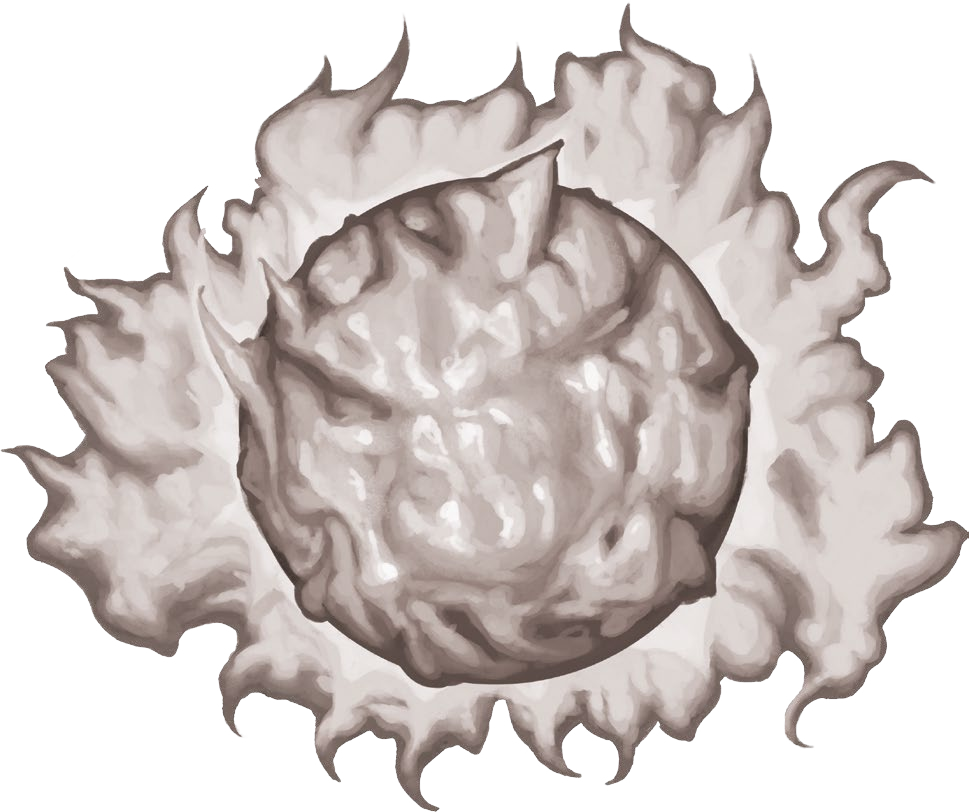
\includegraphics[width=0.85\paperwidth, keepaspectratio]{\art/fireball.png}
  };
  \centering
  \node at (11.5, -2.5) {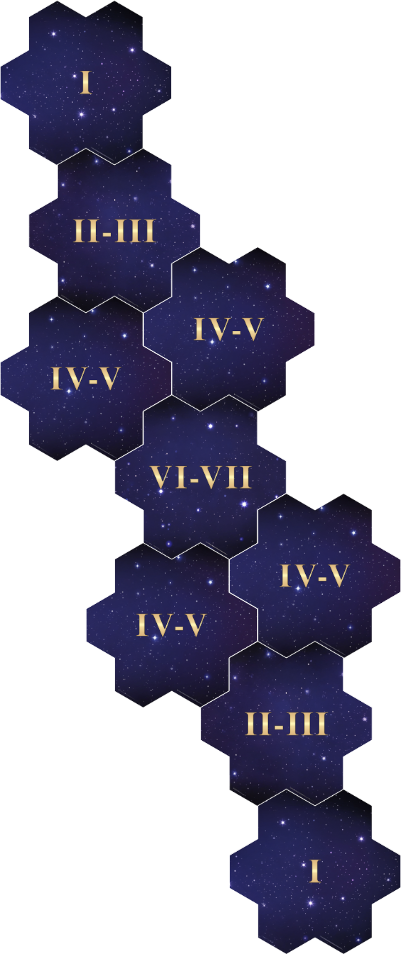
\includegraphics[scale=0.35]{\maps/wandering_dragons_2p.png}};
  \node at (14, -4.9) {\footnotesize{\textbf{\MakeUppercase{2-PLAYER SCENARIO}}}};
  \node at (5.7, -9) {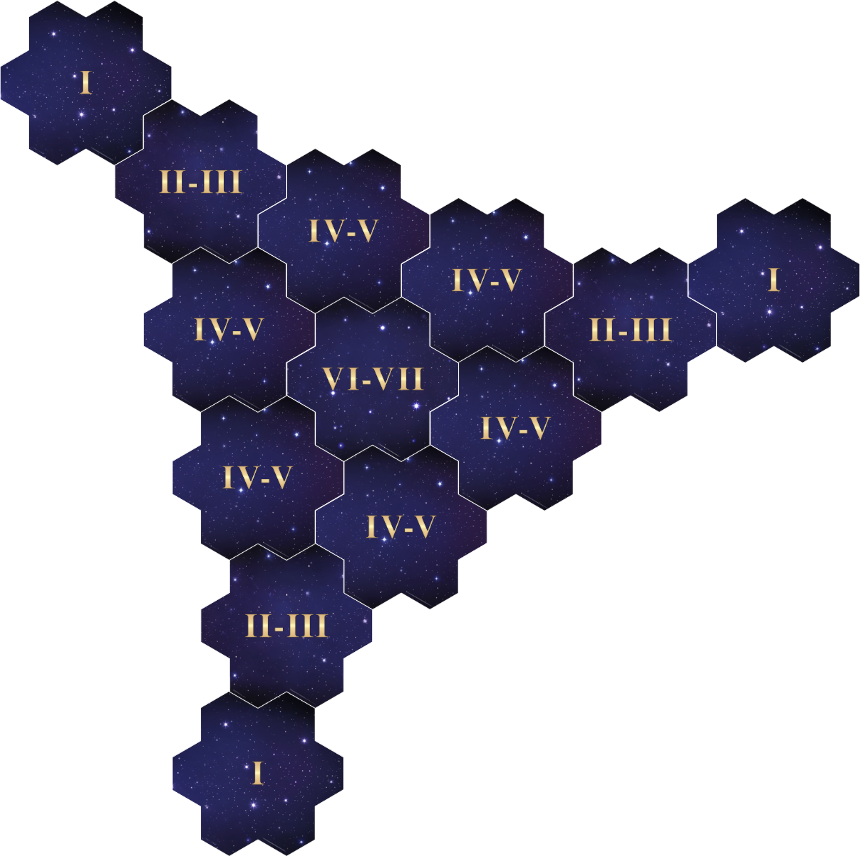
\includegraphics[scale=0.35]{\maps/wandering_dragons_3p.png}};
  \node at (10.5, -9.9) {\footnotesize{\textbf{\MakeUppercase{3-PLAYER SCENARIO}}}};
\end{tikzpicture}
